\chapter{Desenvolvimento}
\label{chap:desenv}

No contexto de DevOps, automação e infraestrutura como código, a ferramenta
proposta por este trabalho, Cupper, propõe auxiliar na extração de configuração
de um ambiente incluso em uma infraestrutura. As configurações extraídas são
transformadas em código em padrões da receita Chef~\ref{fig:cupper_geral}. A
receita gerada é utilizada para qualquer infraestrutura que suporta a
utilização do Chef, como descrito na seção~\ref{sec:chef}.

\begin{figure}[h]
  \centering
  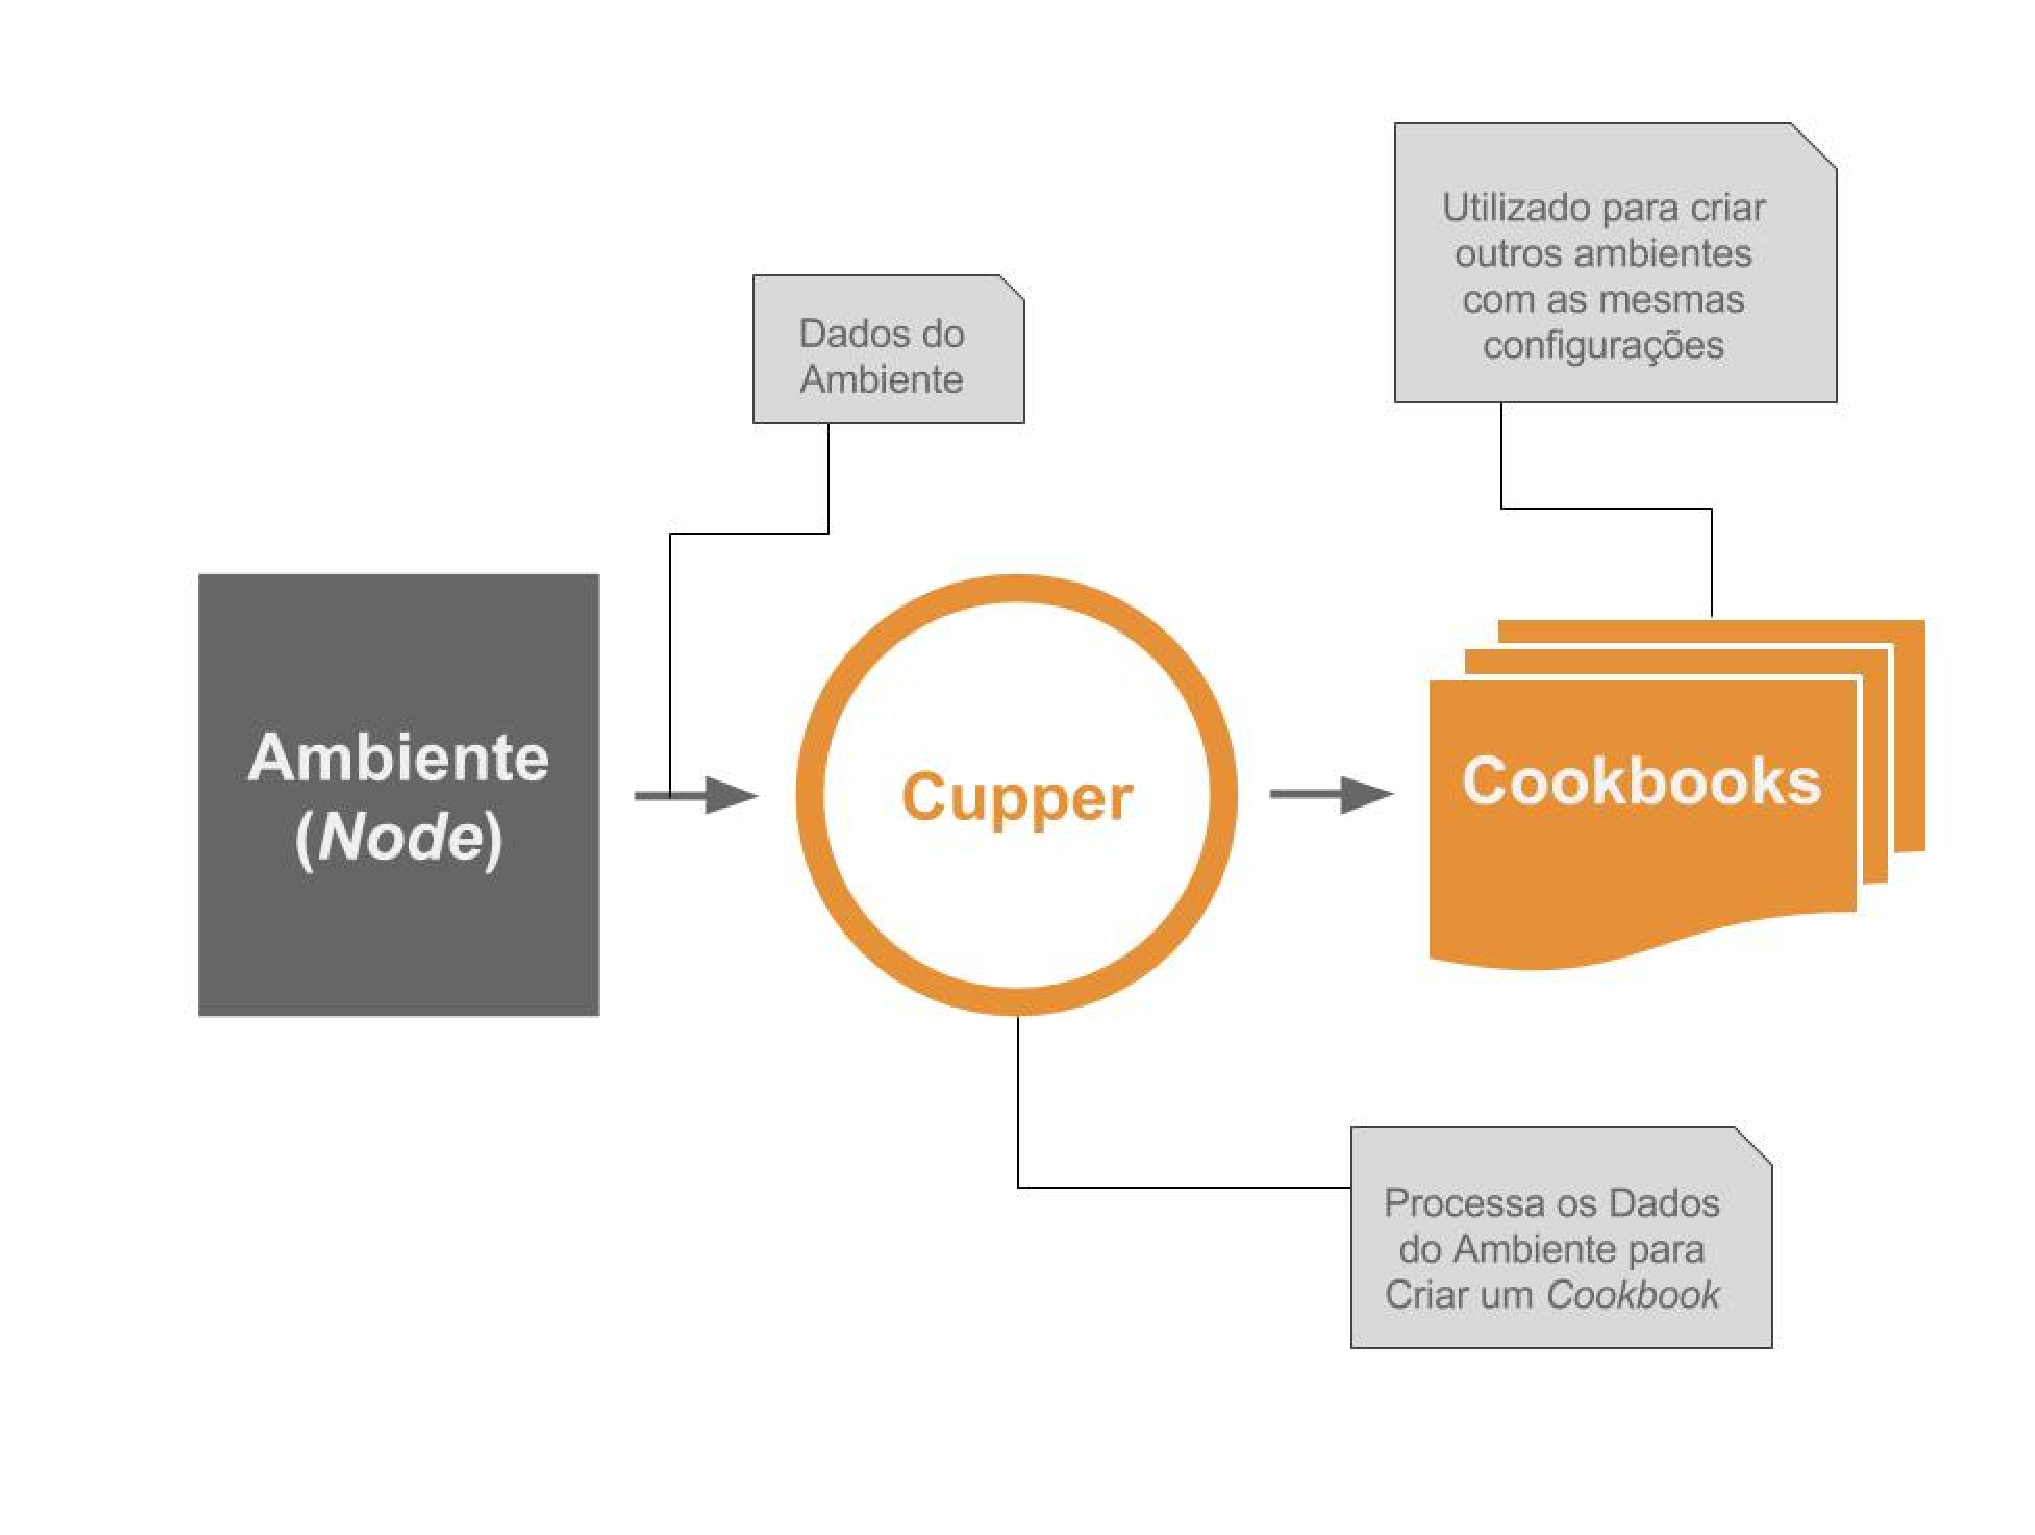
\includegraphics[width=0.8\textwidth]{figuras/cupper_geral.eps}
  \caption{Cupper - Visão geral}
  \label{fig:cupper_geral}
\end{figure}

Além das dependências de desenvolvimento e de \textit{runtime} por ser uma Gem
(\textit{Ruby}, \textit{RubyGems}), o Cupper tem uma dependência muito
importante que é o \textit{Ohai} que é levantado na seção de 
ferramentas~\ref{sec:deps:ohai}. É requisito desse projeto também implementar
\textit{plugins} para que o \textit{Ohai} lance informações que por padrão 
não lança.

As subções seguintes, são mostrados o levantamento dos itens necessários para
a implementação do Cupper, estando organizados em camadas e seus atributos:

\begin{itemize}
  \item \textbf{Camadas de Ambiente}: levantamento e seleção das camadas de ambiente
    e seus atributos necessários a serem coletados;
  \item \textbf{Recursos Chef}: levantamento dos recursos providos pelo Chef e quais os
    itens necessários para a criação de uma receita mínima;
  \item \textbf{Escopo de Implementação}: especificação dos itens a serem implementados
    da ferramenta, abordando até qual ponto a ferramenta Cupper pretende alcançar
    no TCC 2.
\end{itemize}

\section{Camadas de Ambiente}
\label{sec:cam-amb}

As camadas apresentam um conjunto de aspectos do sistema e contém as
informações necessárias que definem o comportamento específico para o
estado desejado daquele ambiente. Os atributos de cada camada são variantes
que são consideradas para o \textit{deployment} de uma aplicação. Sendo assim, as
camadas são dependentes para o nível de compatibilidade da configuração.

\subsection{Levantamento de Camadas de Ambiente}
As seguintes camadas foram definidas para representar o estado de configuração do
sistema:
\begin{itemize}
  \item \textit{\textbf{Hardware}}: definições físicas onde o sistema foi implantado.
    (Arquitetura, memória, espaço em disco, etc);
  \item \textit{\textbf{Operation System}}: definições do sistema operacional
    implantado. Distribuição, arquitetura, versão, etc;
  \item \textit{\textbf{Application}}: definições das aplicações instaladas.
    (Aplicações instaladas, dependências, etc);
  \item \textit{\textbf{Configuration}}: definições das configurações das
    aplicações. (Especificações de implantação de aplicação, arquivos
    de configuração);
  \item \textit{\textbf{Service}}: definições dos serviços daemon que estão em
    funcionamento no sistema.
  \item \textit{\textbf{Custom}}: definições criadas especificamente para o
    sistema sem uma forma padrão conhecida.
\end{itemize}

\subsubsection{\textit{Hardware}}
\label{sec:cam-hard}

A camada de \textit{Hardware} contém as definições físicas do sistema.
As informações são referentes as configurações físicas da máquina, como
CPU, arquitetura, memória, espaço em disco, particionamento, etc. O informe desses atributos
são utilizados para a definição da base do ambiente, ou seja, o sistema
operacional e as aplicações podem ter diferentes desempenhos a partir das
configurações de hardware e/ou apresentar comportamentos inesperados no sistema.
Além das aplicações terem seus requisitos mínimos, algumas são desenhadas
para um tipo específico de arquitetura.

A tabela~\ref{tab:atrhard} mostra diversas informações de hardware possíveis de serem extraídas
do sistema a partir de comandos do sistema operacional e também da ferramenta Ohai, 
dependência prevista para a implementação do Cupper (como descrito na 
seção~\ref{sec:tec}). Nem todas essas informações serão úteis para a 
implementação, mas nessa seção fazemos um levantamento geral antes de fazer uma
seleção.

A camada de hardware será uma das camadas a serem analisadas, e a seleção de 
seus atributos irão seguir os critérios descritos na seção~\ref{sec:defcritcamada}.


\begin{table}[H]
\centering
\caption{Atributos Relacionados a CPU, Memória e \textit{Motherboard}}
\label{tab:atrhard}
\begin{tabular}{|c|c|c|c|l|c|}
\hline
\rowcolor[HTML]{C0C0C0} 
Atributo                                                        & Origem   & Relevante? & Viável? & Ohai & Selecionado? \\ \hline
Modelo CPU                                                      & lscpu    & não        & sim     &      & não          \\ \hline
\begin{tabular}[c]{@{}c@{}}Modo de \\ Operação CPU\end{tabular} & lscpu    & sim        & sim     &      & sim          \\ \hline
Arquitetura CPU                                                 & lscpu    & sim        & sim     &      & sim          \\ \hline
Cores                                                           & lscpu    & sim        & sim     &      & sim          \\ \hline
Stepping CPU                                                    & lscpu    &            & sim     &      &              \\ \hline
Frequência CPU                                                  & lscpu    &            & sim     &      &              \\ \hline
Cache CPU                                                       & lscpu    &            & sim     &      &              \\ \hline
Flags CPU                                                       & lscpu    & sim        & sim     &      & sim          \\ \hline
\begin{tabular}[c]{@{}c@{}}Modelo \\ Motherboard\end{tabular}   & demicode & não        & não     &      & não          \\ \hline
Versão BIOS                                                     & demicode & não        & não     &      & não          \\ \hline
Flags BIOS                                                      & demicode & não        & não     &      & não          \\ \hline
Slots Memória                                                   &          & não        & sim     &      & não          \\ \hline
Marca Memória                                                   & demicode & não        & sim     &      & não          \\ \hline
Tamanho Memória                                                 & free     & sim        & sim     &      & sim          \\ \hline
Clock Memória                                                   &          & sim        & sim     &      & sim          \\ \hline
Total Swap                                                      &          & sim        & sim     &      & sim          \\ \hline
Livre Swap                                                      &          & sim        & sim     &      & sim          \\ \hline
Total Memória                                                   &          & sim        & sim     &      & sim          \\ \hline
Livre Memória                                                   &          & sim        & sim     &      & sim          \\ \hline
Buffers Memóra                                                  &          & não        & sim     &      & não          \\ \hline
Cached Memória                                                  &          &            & sim     &      &              \\ \hline
Ativo Memória                                                   &          &            & sim     &      &              \\ \hline
Inativo Memória                                                 &          &            & sim     &      &              \\ \hline
Sujo Memória                                                    &          &            & sim     &      &              \\ \hline
\begin{tabular}[c]{@{}c@{}}Pag. Anon\\ Memória\end{tabular}     &          &            & sim     &      &              \\ \hline
\end{tabular}
\end{table}

\begin{table}[H]
\centering
\caption{Atributos relacionados a Partições, Armazenamento, USB, PCI, e Rede}
\label{tab:hdmount}
\begin{tabular}{|c|c|c|c|c|l|}
\hline
\rowcolor[HTML]{C0C0C0} 
Atributo                                                                 & Origem                                                                & Relevante? & Viável? & Ohai & Selecionado? \\ \hline
\begin{tabular}[c]{@{}c@{}}Nome\\ dos\\ Dispositivos\end{tabular}        & lsblk                                                                 &            &         &      &              \\ \hline
\begin{tabular}[c]{@{}c@{}}Major/Minor\\ Dispositivos\end{tabular}       & lsblk                                                                 &            &         &      &              \\ \hline
Removíveis                                                               & lsblk                                                                 &            &         &      &              \\ \hline
\begin{tabular}[c]{@{}c@{}}Somente\\ Leitura\end{tabular}                & lsblk                                                                 &            &         &      &              \\ \hline
Partições                                                                & lsblk                                                                 &            &         &      &              \\ \hline
\begin{tabular}[c]{@{}c@{}}Tamanho\\ Partições/\\ Discos\end{tabular}    & \begin{tabular}[c]{@{}c@{}}lsblk/\\ df\end{tabular}                   &            &         &      &              \\ \hline
\begin{tabular}[c]{@{}c@{}}Tipo\\ Filesystem\\ Dispositivos\end{tabular} & lsblk                                                                 &            &         &      &              \\ \hline
\begin{tabular}[c]{@{}c@{}}UUID\\ Dispositivos\end{tabular}              & lsblk                                                                 &            &         &      &              \\ \hline
Mountpoints                                                              & mount                                                                 &            &         &      &              \\ \hline
\begin{tabular}[c]{@{}c@{}}USB\\ Dsipositivos\end{tabular}               & lsusb                                                                 &            &         &      &              \\ \hline
\begin{tabular}[c]{@{}c@{}}PCI\\ Dsipositivos\end{tabular}               & lspci                                                                 &            &         &      &              \\ \hline
\begin{tabular}[c]{@{}c@{}}Rede\\ Dispositivos\end{tabular}              & \begin{tabular}[c]{@{}c@{}}lspci/\\ ifconfig/\\ demicode\end{tabular} &            &         &      &              \\ \hline
\end{tabular}
\end{table}

{\color{red} colocar uma tabela com saida dos comandos lscpu, lshw, hwinfo, lspci
lsscsi, lsusb, lsblk, df, mount, free, e ohai}

{\color{red} explicar de onde vem cada informação, e cada comando}

{\color{red} tirar o que for redundante}

%TODO: adicionar as informações que serão coletadas.

\subsubsection{\textit{Operation System}}
\label{sec:cam-os}

A segunda camada de extração de dados é a do Sistema Operacional. 
Cada sistema tem a sua particularidade com relação aos gerenciamento dos 
recursos de hardware e administração de processos. Portanto é necessário a 
construção de uma arquitetura flexível, que contenha os aspectos em comum aos
sistemas operacionais, e modular para que seja possível escalar a utilização 
da ferramenta para mais Sistemas Operacionais.

Inicialmente a ferramenta Cupper irá abordar dois sistemas operacionais, 
ambos baseados em GNU/Linux: Archlinux e Debian.

A tabela~\ref{} mostra informações a respeito do Kernel e da distribuição
analisada extraídas a partir de comandos do próprio sistema ou do Ohai.


{\color{red} tabela com infos de distro, versões, pkg manager tool, e kernel do ohai}

{\color{red} detectar qual init system é usado verificando existência de diretórios
e outros métodos}

{\color{red} extrair qual sistema de segurança é usado verificando existência
do apparmour, selinux ou grsecurity}

{\color{red} explicar de onde veio cada dado}

%TODO: a seleção de camadas e profundidade de análise serão postas dentro das
%   especificações de cada camada.


\section{Recursos Chef}
\label{sec:lev-rec}

Como descrito ne seção \ref{sec:chef}, o Chef é disposto em vários
componentes. O foco principal do Cupper é a criação de \textit{cookbooks},
sendo assim os recursos levantados são referente a composição interna
dos \textit{cookbooks}.

Os \textit{cookbooks} contém os seguintes componentes: \textit{attributes, recipes, definitions,
files, libraries, custom resourses, metadata, resources e providers, templates
cookbook versions}~\cite{chefdoc:2016}.

Para o funcionamento de um \textit{cookbook}, com uma estrutura mínima, é necessário que tenha
ao menos um \textit{recipe default} definido. O exemplo \ref{code:tree} mostra essa
estrutura mínima necessária para realizar a configuração do \textit{cookbook app}.

\noindent\begin{minipage}{.9\textwidth}
  %\lstset{style=shell}
  \lstinputlisting[language=Bash, label=code:tree, caption="Estrutura mínima de um cookbook"]{conteudo/code/minimal_tree}
\end{minipage}\hfill

As subseções seguintes explicam os componentes dos \textit{cookbooks} e quais serão gerados
pelo Cupper.

\subsection{\textit{Attributes}}
\label{sec:lev-rec-att}

Os \textit{attributes} são os detalhes das especificações do \textit{node}. Definem~\cite{chefdoc:2016}:

\begin{itemize}
  \item o estado atual do \textit{node};
  \item em qual estado o \textit{node} estava após a última execução do \textit{chef-client};
  \item em qual estado o \textit{node} deve alcançar ao final na execução do \textit{chef-client} atual.
\end{itemize}

Os \textit{attributes} são definidos: no proprio ambiente através do Ohai, nos \textit{cookbooks},
nos \textit{roles} e \textit{environments}.

\textbf{Cupper}:

\subsection{\textit{Recipes}}
\label{sec:lev-rec-rec}

Os \textit{recipes} são as unidade fundamentais para a execução de um \textit{cookbook}. Definem
todas as informações necessárias para configurar o sistema e segue algumas regras
~\cite{chefdoc:2016}:

\begin{itemize}
  \item Deve ser incluido em um \textit{cookbook};
  \item Deve ser posto em um \textit{run-list} antes de ser usado pelo \textit{chef-client};
  \item É executado na mesma ordem disposta na \textit{run-list};
  \item Pode ser incluído em outro \textit{recipe};
  \item Pode ter dependência de outros \textit{recipe};
  \item Pode marcar um \textit{node} para facilitar a criação de agrupamento.
\end{itemize}

As \textit{recipes} são escritas em Ruby e pode-se utilizar dos recursos providos
pela linguagem. Dispoem-se de uma coleção desse recursos que são utilizados
para definir as ações da \textit{recipes}. No exemplo \ref{code:recipe} utiliza-se
três recursos: \textit{package, service} e \textit{template}.

\begin{minipage}{.90\textwidth}
  \lstset{style=shell}
  \lstinputlisting[language=Bash, label=code:recipe, caption="Exemplo de \textit{recipe}. Define a instala{\c{c}}{\~a}o e configura{\c{c}}{\~a}o do \textit{app} Nginx"]{conteudo/code/recipe_example.rb}
\end{minipage}

\textbf{Cupper}:

\subsection{\textit{Definitions}}
\label{sec:lev-rec-def}

As \textit{definitions} são um novo tipo de recurso disponível apartir da versão
12.5 do Chef e é recomentado utilizar o \textit{Custom Resource}(seção \ref{sec:lev-rec-cust})
no lugar de \textit{definitions}~\cite{chefdoc:2016}.

Os \textit{definitions} são comportamento que podem ser reutilizados por outros \textit{recipes}.
São utilizado como recursos padrões de uma receita. No exemplo \ref{code:definition}
é definido o recurso \textit{host\_porter} com os parametros \textit{port} (valor padrão 4000)
e \textit{hostname} (valor padrão \textit{nil}) que pode ser utilizado em outro
\textit{recipe} com a simples chamada \textit{host\_porter}.

\begin{minipage}{.90\textwidth}
  \lstset{style=shell}
  \lstinputlisting[language=Bash, label=code:definition, caption="Exemplo de \textit{definition}. Adiciona um recurso \textit{host\_porter}."]{conteudo/code/definition_example.rb}
\end{minipage}

\textbf{Cupper}:

\subsection{\textit{Files}}

\textbf{Cupper}:

\subsection{\textit{Libraries}}

\textbf{Cupper}:

\subsection{\textit{Custom Resource}}
\label{sec:lev-rec-cust}

\textbf{Cupper}:

\subsection{\textit{Metadata}}

\textbf{Cupper}:

\subsection{\textit{Resources e Providers}}

\textbf{Cupper}:

\subsection{\textit{Templates}}

\textbf{Cupper}:

\subsection{\textit{Cookbook Version}}

\textbf{Cupper}:

\section{Relação entre Camadas e \textit{Cookbooks}}



\section{Escopo de Implementação}
\label{sec:escopo}
Nessa seção serão descritas as funcionalidades e a estrutura inicial da gem.

\subsection{Funcionalidades}



\subsection{Estrutura e módulos}

\begin{figure}[H]
  \centering
  \includegraphics[width=1.05\textwidth]{figuras/cupper_detail.eps}
  \caption{Estrutura Inicial Planejada para os Módulos do Cupper}
  \label{fig:cupper-detail}
\end{figure}



\subsection{Criação de \textit{Cookbooks}}

